\documentclass[11pt]{article}
\usepackage[letterpaper,margin=0.7in]{geometry}
\usepackage[T1]{fontenc}
\usepackage{lmodern,microtype}
\usepackage{amsmath,amssymb,booktabs,tabularx,array}
\usepackage{tikz}
\usetikzlibrary{arrows.meta,positioning,calc}
\usepackage{xurl}
\usepackage[colorlinks=true,urlcolor=blue!45!black,linkcolor=blue!45!black]{hyperref}
\usepackage{enumitem}
\setlist[enumerate]{leftmargin=*,itemsep=1pt,topsep=3pt}
\setlength{\parindent}{0pt}
\setlength{\parskip}{4pt}
\setlength{\abovedisplayskip}{5pt}
\setlength{\belowdisplayskip}{5pt}
\emergencystretch=2em
\newcommand{\file}[1]{\nolinkurl{#1}}
\newcommand{\heading}[1]{\vspace{4pt}{\large\bfseries #1}\par}
\newcolumntype{Y}{>{\raggedright\arraybackslash}X}
\begin{document}
{\LARGE\bfseries Lean-in-the-loop RL: training setup}\par
{\large RL course presentation brief}\hfill 11 October 2026\par

The question is whether reinforcement learning (RL) improves complete, unassisted number-theory proofs after supervised fine-tuning (SFT).
Training is stopped. The earlier CPU engineering smoke remains isolated from future initialization.
Prerequisite competence, GPU throughput, and improved proof success remain unverified.

\heading{1. Reuse assessments; prepare prerequisites}
Earlier assessments exist. The saved interactive baseline failed format checks before Lean; it cannot establish capability after the parser correction.
Audit parent and settings before reuse.
The new frozen, no-update high-school diagnostic is prepared but unrun.

The prepared corpus uses GSM8K and MATH training splits, with separate internal development (DEV) data.
Exact grouping and lexical exclusions control duplicates; they do not establish semantic independence.
The order starts with arithmetic, then balances MATH subjects within competition difficulty levels.
These levels are not school grades or validated prerequisites.
Policy prompts contain questions; private solutions remain scorer targets with reserved context space.

Optional reinforcement as a pretraining objective (RLP) scores private solution log-likelihood gain after sampled reasoning, relative to an exponential moving average teacher without that reasoning.
The warm-up is unauthorized.
Likelihood gain does not certify answer correctness or transfer to Lean.

\heading{2. Separate a proof path from a training trajectory}
The implemented loop in Figure~\ref{fig:loop} admits checked tactics into the proof path.
Rejected actions remain outside that path.
Their original token likelihoods and penalties remain in the training trajectory.

\begin{center}
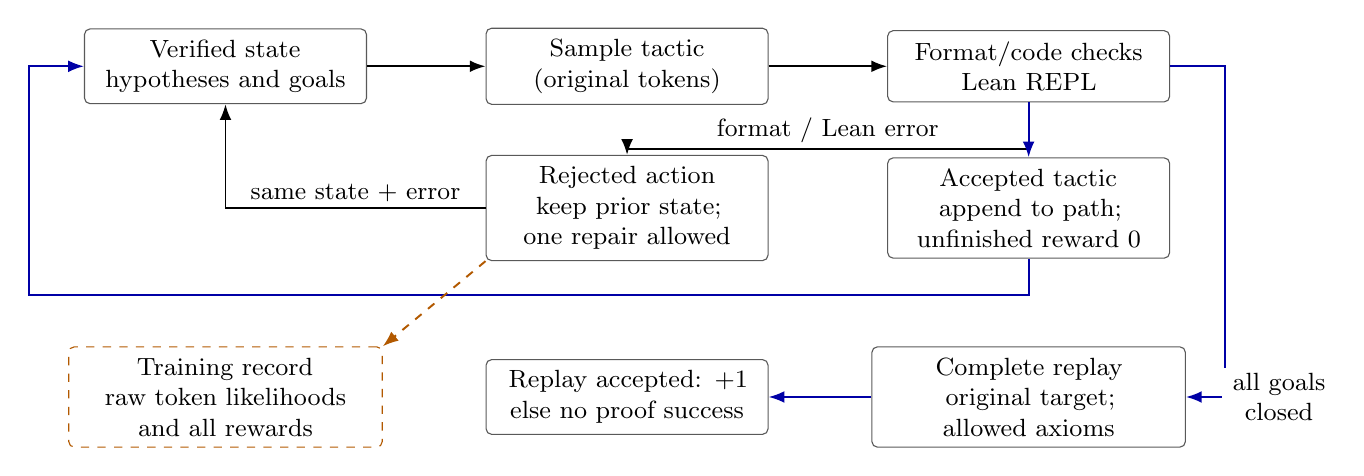
\begin{tikzpicture}[
  box/.style={draw=black!65,rounded corners=2pt,align=center,text width=3.3cm,minimum height=0.8cm,inner sep=4pt,font=\small},
  flow/.style={-{Latex[length=2mm]},line width=0.7pt},
  verified/.style={flow,draw=blue!65!black},
  record/.style={flow,dashed,draw=orange!70!black},
  lab/.style={font=\small,fill=white,inner sep=2pt,align=center}
]
\node[box] (state) at (0,0) {Verified state\\hypotheses and goals};
\node[box] (policy) at (5.1,0) {Sample tactic\\(original tokens)};
\node[box] (check) at (10.2,0) {Format/code checks\\Lean REPL};
\node[box] (reject) at (5.1,-1.8) {Rejected action\\keep prior state;\\one repair allowed};
\node[box] (advance) at (10.2,-1.8) {Accepted tactic\\append to path;\\unfinished reward $0$};
\node[box,text width=3.7cm] (replay) at (10.2,-4.2) {Complete replay\\original target;\\allowed axioms};
\node[box] (terminal) at (5.1,-4.2) {Replay accepted: $+1$\\else no proof success};
\node[box,dashed,draw=orange!70!black,text width=3.7cm] (trace) at (0,-4.2) {Training record\\raw token likelihoods\\and all rewards};
\draw[flow] (state) -- (policy);
\draw[flow] (policy) -- (check);
\draw[flow] (check.south) -- (10.2,-1.05) -- node[lab,above]{format / Lean error} (5.1,-1.05) -- (reject.north);
\draw[flow] (reject.west) -- node[lab,above]{same state + error} (0,-1.8) -- (state.south);
\draw[verified] (check) -- (advance);
\draw[verified] (advance.south) -- (10.2,-2.9) -- (-2.5,-2.9) |- (state.west);
\draw[verified] (check.east) -- ++(0.7,0) |- node[lab,pos=0.55,right,text width=1.3cm]{all goals closed} (replay.east);
\draw[verified] (replay) -- (terminal);
\draw[record] (reject.south west) -- (trace.north east);
\end{tikzpicture}
\end{center}
\vspace{-5pt}
{\small\refstepcounter{figure}\label{fig:loop}\textbf{Figure \thefigure.}
Blue arrows carry accepted states or complete-proof checks; the dashed arrow records rejected actions.
Repairs consume existing caps.
Forbidden code, repeated states, infrastructure failures, and rejected replay stop without repair.}

\textbf{Conditional correctness.}
Closing REPL goals alone is insufficient.
Complete replay requires one theorem command with the original target and permits only \file{propext}, \file{Classical.choice}, and \file{Quot.sound}.
Assuming the pinned Lean kernel and verifier checks operate correctly, acceptance certifies a proof of that formal target under those axioms.
It does not prove implementation soundness, strategy, or learning.

\newpage
{\Large\bfseries Objective, controls, and next work}\par
\heading{3. Use the implemented policy update}
Let $s_{it}$ be the verified goals plus any repair diagnostic for trajectory $i$ at action $t$.
Let $a_{it}$ contain the original sampled tokens, including end-of-sequence when sampled.
The feedback arm uses:

\begin{tabularx}{\linewidth}{@{}lY@{}}
\toprule
Reward & Outcome \\
\midrule
$+1$ & Complete replay accepted by target and axiom checks (Lean-verified). \\
$-0.2$ & Format, syntax, forbidden-code, or classified unresolved-name failure (heuristic). \\
$-0.1$ & Classified type/tactic failure or rejected complete replay (heuristic). \\
$0$ & Valid unfinished action, repeated state, unclassified or infrastructure failure. \\
\bottomrule
\end{tabularx}

The terminal-only control assigns zero to every nonterminal outcome.
Neither arm rewards changed goals or valid unfinished tactics.
Error categories and weights are heuristic; they change the objective without an optimal-policy-preservation claim.
Improved return can reflect fewer invalid actions without more proofs.

For $G\geq2$ independent trajectories from one root, with lengths $T_i$ and rewards $r_{iu}$, define
\begin{align*}
R_{it}&=\sum_{u=t}^{T_i}r_{iu},
& b_i&=\frac{1}{G-1}\sum_{j\ne i}\sum_{u=1}^{T_j}r_{ju},
& A_{it}&=R_{it}-b_i,\\
L(\theta)&=-\frac{1}{G}\sum_{i=1}^{G}\sum_{t=1}^{T_i}
\operatorname{stopgrad}(A_{it})\log\pi_\theta(a_{it}\mid s_{it}).
\end{align*}
Here $\operatorname{stopgrad}$ fixes the advantage during differentiation.
The update uses on-policy REINFORCE with reward-to-go and the other trajectories' mean total return as its baseline.
The interactive trainer uses neither PPO nor GRPO.
Likelihood sums the original token log probabilities; parsing never retokenizes the training action.
Sampling and replay use the same unwarped policy with dropout disabled.

\heading{4. Hold the comparison fixed}
Both prepared reward arms share the immutable common-SFT parent, task bank, seed, optimizer, retry allowance, and resource caps.
Training mixes whole roots and short assisted prefixes; evaluation supplies no proof prefix.
Settings are prepared, not optimized.
Lean is pinned to \file{v4.10.0-rc1}; mathlib to \file{29dcec074de168ac2bf835a77ef68bbe069194c5}.

Historical SFT/RLP and SFT/GRPO interleaving includes extra SFT refreshes, preventing RL-only attribution.
The prepared pair compares error feedback with terminal-only reward.
Complete, unassisted proof success is the endpoint; search efficiency is deferred.
Select checkpoints and task mixes on DEV only; held-out tests remain untouched.
Report generated tokens, physical Lean calls, and wall time beside success.
The existing \file{gpu_seconds} field is a CUDA wall-time proxy.

\heading{5. Follow the dependencies}
\begin{enumerate}
\item Audit and reuse matched saved baselines. Fill unmatched coverage with the frozen, no-update diagnostic.
\item Use diagnosed weaknesses to decide whether prerequisite warm-up is needed.
\item Measure hardware throughput and memory before fixing the feasible budget.
\item After launch approval, run the matched reward comparison.
\item Evaluate both arms and the unchanged parent with identical inference budgets.
\end{enumerate}
A claim that RL beats SFT also needs matched continued SFT.
That control is recommended, not implemented in this pair.
This document authorizes no training or compute spend.

\vfill
{\small\textbf{Sources.}
\file{README.md}; \file{docs/EXPERIMENTS.md}, EXP-019/020.\\
Code:
\href{../../scripts/train/run_tactic_rl.py}{\texttt{run\_tactic\_rl.py}},
\href{../../scripts/train/run_rlp_pilot.py}{\texttt{run\_rlp\_pilot.py}},
\href{../../scripts/eval/bench_lean_verifier.py}{\texttt{bench\_lean\_verifier.py}}.
\href{https://lean-lang.org/theorem_proving_in_lean4/Axioms-and-Computation/}{Lean axioms};
\href{https://tikz.dev/tikz-arrows}{TikZ notation}.}
\end{document}
